% Instructions to change to html version:
% Comment out:
%  minipage, multicols,columnbreak, mathbf, hrule
% Replace all: \begin{minipage}% \end{minipage} %\begin{multicols}  %\end{multicols}  %\columnbreak %% \begin{framed} %\end{framed} %%\hrule
% Replace \mathbf with \boldsymbol
% Replace $$ with \[ or \]and $ with \( or \)
% Enclose graphics in figure environments and add captions
% 			search \includegraphics
% Re-tag \df environments as sections, subsections, etc.
% Command Line Code to Create html version:
%First: pdflatex -shell-escape filename.tex                                   
%Second, for each figure: inkscape "filename-figure1.pdf" -o "filename-figure1.png"
% Third: htlatex filename.tex "ht5mjlatex.cfg, charset=utf-8" " -cunihtf -utf8"

\documentclass[10pt]{article}

%\usepackage{tikz, pgf,pgfplots,wasysym,array}
%\usepackage{wasysym,array}

\usepackage{amsmath,amssymb}

\ifdefined\HCode
  \def\pgfsysdriver{pgfsys-tex4ht-updated.def}
\fi 
%\ifdefined\HCode
%  \def\pgfsysdriver{pgfsys-dvisvgm4ht.def}
%\fi 
\usepackage{tikz}
\usetikzlibrary{calc,decorations.markings,arrows}
\usepackage{pgfplots}

\pgfplotsset{compat=1.12}
\usepackage{myexternalize}
\usetikzlibrary{calc,decorations.markings,arrows}
\usepackage{framed}
\usepackage[none]{hyphenat}

\input{../../../common/1336_header_test.tex}
\begin{document}

\everymath{\displaystyle}


\newcommand{\ihat}{\boldsymbol{\hat{\textbf{\i}}}}
\newcommand{\jhat}{\boldsymbol{\hat{\textbf{\j}}}}
\newcommand{\khat}{\boldsymbol{\hat{\textbf{k}}}}

\let\oldvec\vec
\renewcommand{\vec}[1]{\oldvec{\boldsymbol{#1}}}

\renewcommand{\u}{\vec{u}}
\renewcommand{\v}{\vec{v}}
\newcommand{\w}{\vec{w}}
\renewcommand{\r}{\vec{r}}
\renewcommand{\a}{\vec{a}}
\renewcommand{\b}{\vec{b}}

\newcommand{\<}{\left\langle}
\renewcommand{\>}{\right\rangle}

\renewcommand{\myTitle}{MATH 1336: Calculus III}

\renewcommand{\mySubTitle}{Section 3.3: %Vector Functions, Space Curves, \& Arclength}%, 
%\& 
TNB Frame \vspace*{-.2in}}
%~\hfill Name: \underline{~~~~~~~~~~~~~~~~~~~~~~~~~~~~~~~~~~~~~~~~~~~~~~~}

\lectTitle{\vspace*{-.5in}\myTitle}{\vspace*{.1in}\mySubTitle \vspace*{-.2in}}


\setlength{\columnseprule}{0.4pt}
\setlength{\columnsep}{3em}


\section*{TNB Frame:}


%\begin{framed}
At any point on a smooth curve, \(\vec{r}(t)\), where \(\vec{T}\ '(t) \neq \vec{0}\), we can define the following set of vectors. %, which form the \textbf{TNB Frame}. 
Note that these vectors all have unit length, and are all mutually orthogonal. 
\vspace*{.2in}

%\begin{minipage}{.5\textwidth}

\begin{figure}[!h]
\centering
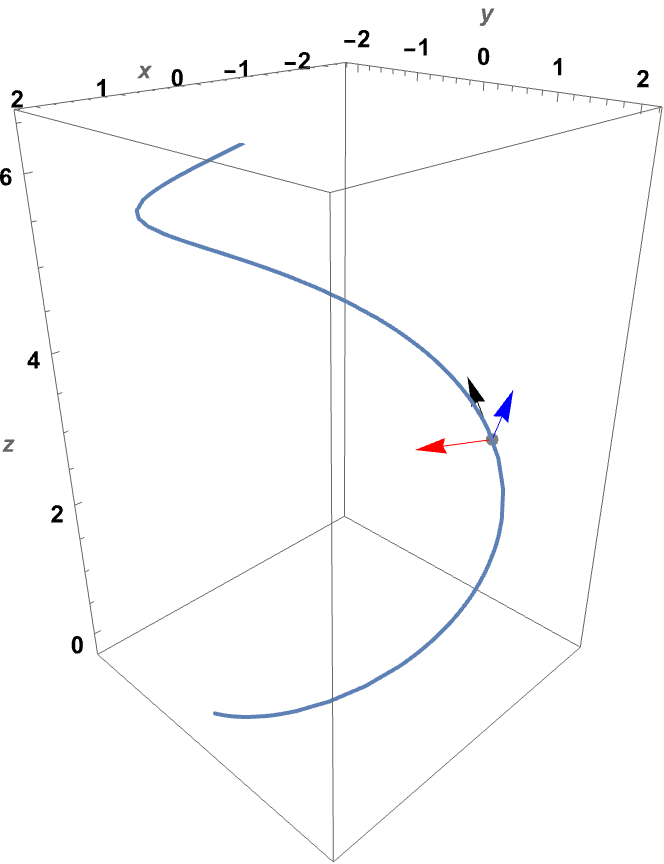
\includegraphics[width=.75\textwidth]{TNBplot.png}
\caption{TNB Frame plotted at a point along the helix from the Chapter 3, Part 1 Worksheet.}
\end{figure}

%\end{minipage}
\hspace*{-.5in}
%\begin{minipage}{.5\textwidth}

Unit Tangent Vector:
\[
\vec{T}(t) = \frac{\vec{r}\ '(t)}{\Vert\vec{r}\ '(t)\Vert} 
\]

Unit Normal Vector:
\[
\vec{N}(t) = \frac{\vec{T}\ '(t)}{\Vert\vec{T}\ '(t)\Vert} 
\]

Binormal Vector:
\[
\vec{B}(t) = \vec{T}(t) \times \vec{N}(t)
\]

%\end{minipage}

~\\
The \textbf{TNB Frame}, also known as the \textbf{Frenet frame of reference}, is the the three-dimensional frame of reference formed by the unit tangent vector, \(\vec{T}\), the unit normal vector, \(\vec{N}\), and the binormal vector, \(\vec{B}\). They form a moving reference frame at any point on a given smooth curve.\\

Note that the \textbf{osculating circle} lies in the plane determined by the vectors \(\vec{T}\) and \(\vec{N}\).

%\end{framed}


\begin{flushright}
\textit{(See Mathematica demonstration)}
\end{flushright}

%\newcounter{prob}
%\begin{list}{\bf{Example \arabic {prob}: }}{\usecounter{prob}}
%
%\item Show that the curvature of a line is zero!\\
%Hint: the equation for a generic line is \(\vec{r}(t) = <x_0+at, y_0+bt, z_0+ct>\)
%
%\vfill
%
%\item Show that the curvature of the helix \(\vec{r}(t) = \<R \cos t, R \sin t, \alpha t\>\) is \(\kappa = \dfrac{R}{R^2+\alpha^2}\)
%\begin{enumerate}[(a)]
%\item Using the formula \(\kappa = \dfrac{\Vert\vec{T}\ '(t)\Vert}{\Vert\vec{r}\ '(t)\Vert}\)
%\item Using the formula \(\kappa = \dfrac{\Vert\vec{r}\ '(t) \times \vec{r}\ ''(t)\Vert}{\Vert\vec{r}\ '(t)\Vert^3}\)
%\item Which way was easier?
%\end{enumerate}
%
%\vfill
%
%\pagebreak
%
%
%
%\end{list}

\end{document}
